\documentclass{standalone}
\usepackage{tikz}
\usetikzlibrary{patterns, positioning}
\usepackage[sfdefault]{ClearSans} %% option 'sfdefault' activates Clear Sans as the default text font
\usepackage[T1]{fontenc}

\begin{document}
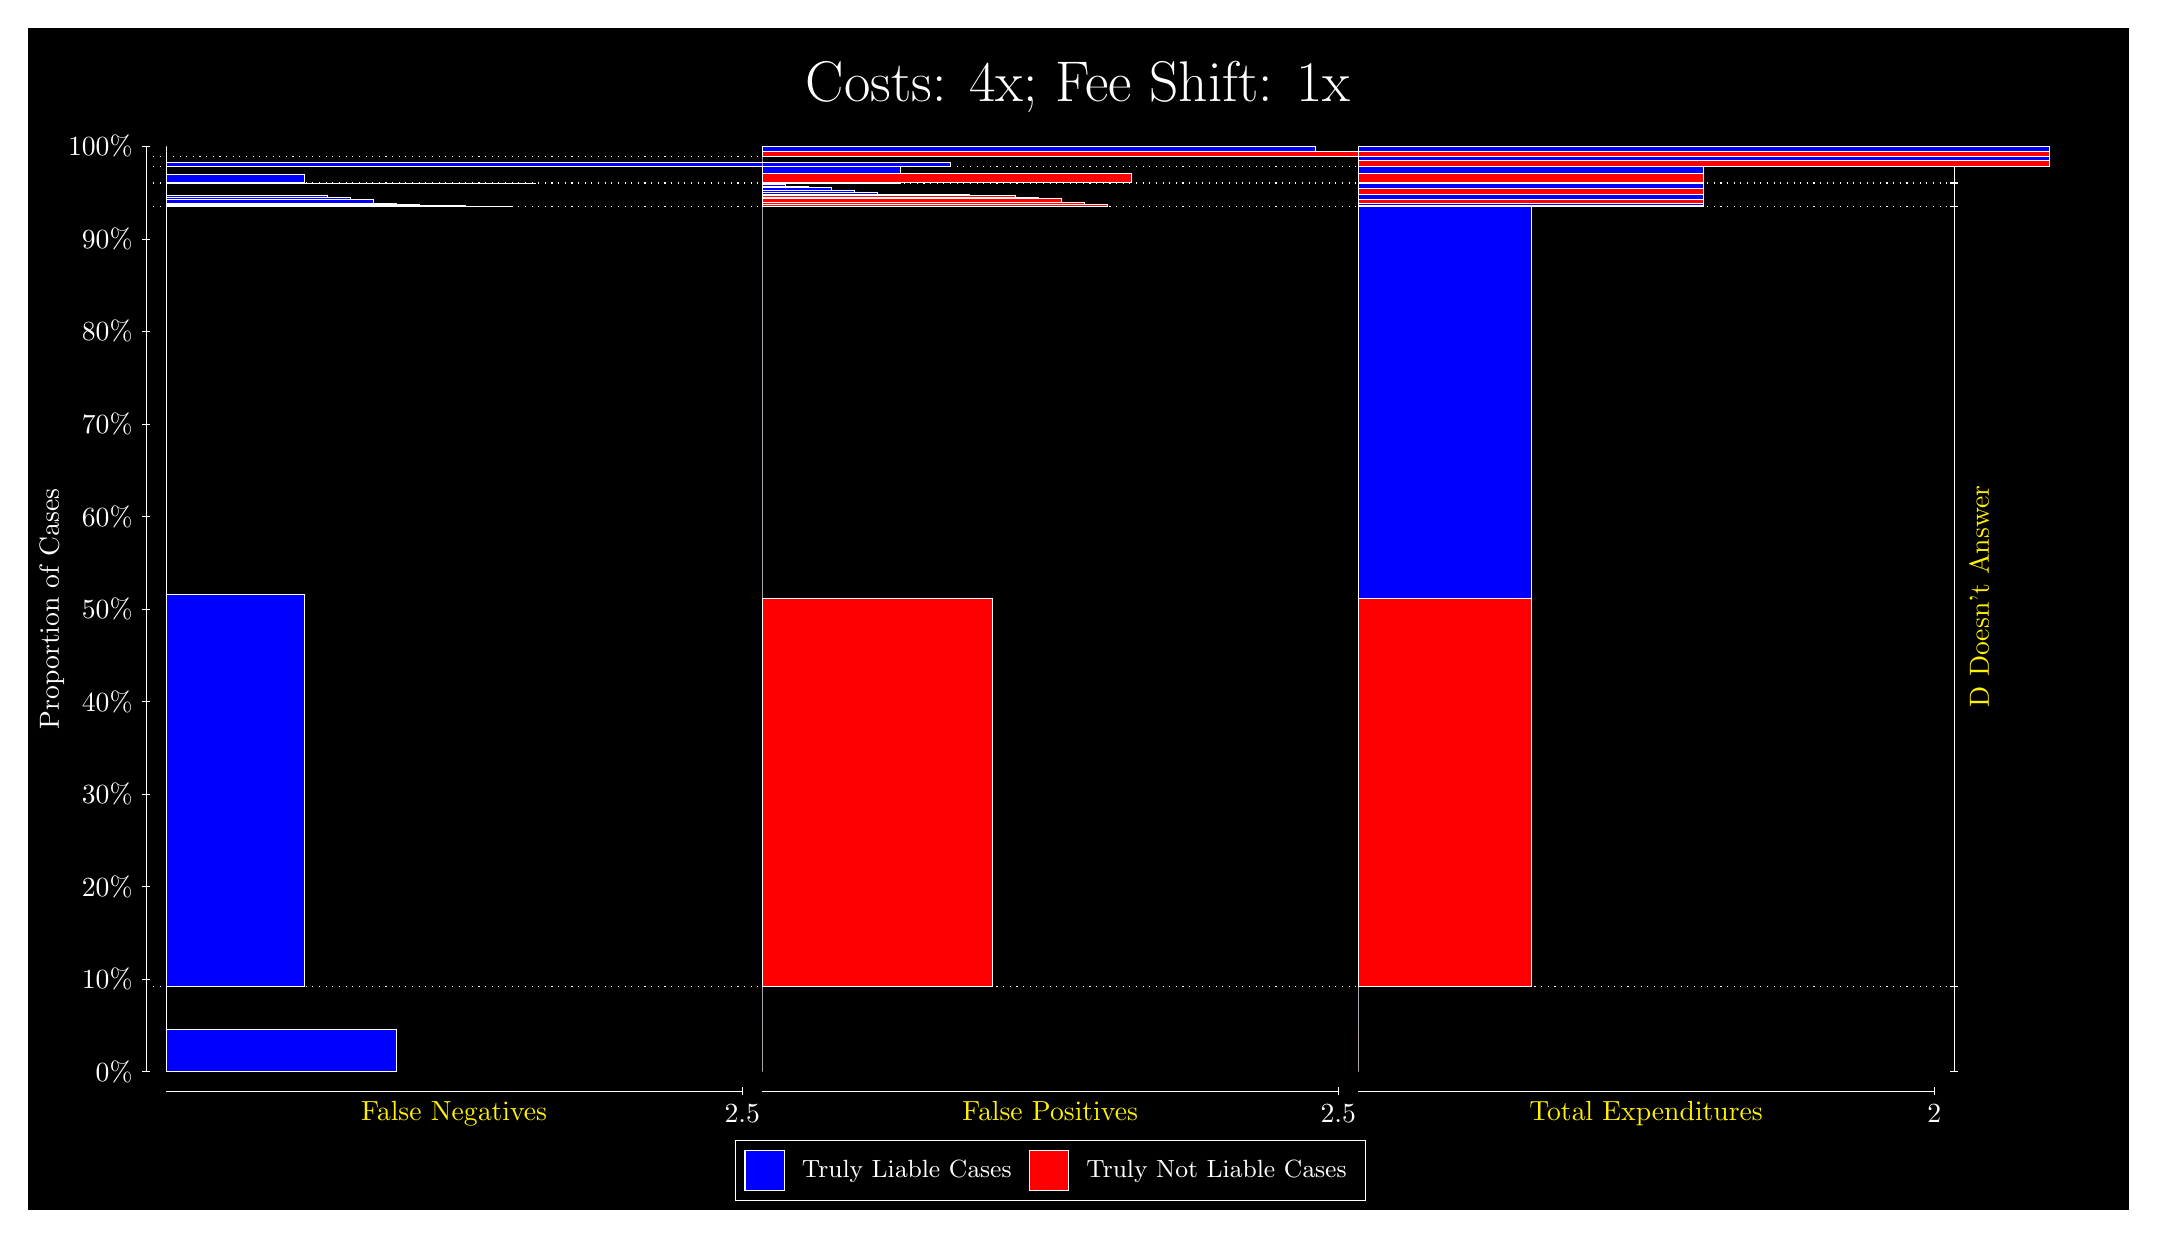
\begin{tikzpicture}
\draw[fill=black] (0,0) rectangle (26.667,15);
\draw[text=white] (0,13.5) rectangle (26.667,15) node[midway] {\huge Costs: 4x; Fee Shift: 1x};
\draw[white, very thin] (1.5,1.75) -- (1.5,13.5);
\node[rotate=90, text=white, anchor=center] at (0.3, 7.625) {Proportion of Cases};
\draw[white, very thin] (1.45,1.75) -- (1.55,1.75);
\node[text=white, anchor=east] at (1.45, 1.75) {0\%};
\draw[white, very thin] (1.45,2.925) -- (1.55,2.925);
\node[text=white, anchor=east] at (1.45, 2.925) {10\%};
\draw[white, very thin] (1.45,4.1) -- (1.55,4.1);
\node[text=white, anchor=east] at (1.45, 4.1) {20\%};
\draw[white, very thin] (1.45,5.275) -- (1.55,5.275);
\node[text=white, anchor=east] at (1.45, 5.275) {30\%};
\draw[white, very thin] (1.45,6.45) -- (1.55,6.45);
\node[text=white, anchor=east] at (1.45, 6.45) {40\%};
\draw[white, very thin] (1.45,7.625) -- (1.55,7.625);
\node[text=white, anchor=east] at (1.45, 7.625) {50\%};
\draw[white, very thin] (1.45,8.8) -- (1.55,8.8);
\node[text=white, anchor=east] at (1.45, 8.8) {60\%};
\draw[white, very thin] (1.45,9.975) -- (1.55,9.975);
\node[text=white, anchor=east] at (1.45, 9.975) {70\%};
\draw[white, very thin] (1.45,11.15) -- (1.55,11.15);
\node[text=white, anchor=east] at (1.45, 11.15) {80\%};
\draw[white, very thin] (1.45,12.325) -- (1.55,12.325);
\node[text=white, anchor=east] at (1.45, 12.325) {90\%};
\draw[white, very thin] (1.45,13.5) -- (1.55,13.5);
\node[text=white, anchor=east] at (1.45, 13.5) {100\%};

\draw[white, very thin] (24.457,1.75) -- (24.457,13.5);
\draw[white, very thin] (24.407,1.75) -- (24.507,1.75);
\node[anchor=west] at (24.407, 1.75) {};
\draw[white, very thin] (24.407,2.8353) -- (24.507,2.8353);
\node[anchor=west] at (24.407, 2.8353) {};
\draw[white, very thin] (24.407,12.736) -- (24.507,12.736);
\node[anchor=west] at (24.407, 12.736) {};
\draw[white, very thin] (24.407,13.029) -- (24.507,13.029);
\node[anchor=west] at (24.407, 13.029) {};
\draw[white, very thin] (24.407,13.044) -- (24.507,13.044);
\node[anchor=west] at (24.407, 13.044) {};
\draw[white, very thin] (24.407,13.247) -- (24.507,13.247);
\node[anchor=west] at (24.407, 13.247) {};
\draw[white, very thin] (24.407,13.375) -- (24.507,13.375);
\node[anchor=west] at (24.407, 13.375) {};
\draw[white, very thin] (24.407,13.5) -- (24.507,13.5);
\node[anchor=west] at (24.407, 13.5) {};

\draw[white, very thin, fill=blue] (1.75,1.75) rectangle (4.6775,2.2926);
\draw[white, very thin, fill=red] (1.75,2.2926) rectangle (1.75,2.8353);
\draw[white, very thin, fill=blue] (1.75,2.8353) rectangle (3.5065,7.8111);
\draw[white, very thin, fill=red] (1.75,7.8111) rectangle (1.75,12.736);
\draw[white, very thin, fill=blue] (1.75,12.736) rectangle (6.1413,12.738);
\draw[white, very thin, fill=blue] (1.75,12.738) rectangle (5.8486,12.741);
\draw[white, very thin, fill=blue] (1.75,12.741) rectangle (5.5558,12.747);
\draw[white, very thin, fill=blue] (1.75,12.747) rectangle (5.2631,12.752);
\draw[white, very thin, fill=blue] (1.75,12.752) rectangle (4.9703,12.769);
\draw[white, very thin, fill=blue] (1.75,12.769) rectangle (4.6775,12.783);
\draw[white, very thin, fill=blue] (1.75,12.783) rectangle (4.3848,12.822);
\draw[white, very thin, fill=blue] (1.75,12.822) rectangle (4.092,12.848);
\draw[white, very thin, fill=blue] (1.75,12.848) rectangle (3.7993,12.872);
\draw[white, very thin, fill=red] (1.75,12.872) rectangle (1.75,13.029);
\draw[white, very thin, fill=blue] (1.75,13.029) rectangle (6.4341,13.036);
\draw[white, very thin, fill=red] (1.75,13.036) rectangle (1.75,13.044);
\draw[white, very thin, fill=blue] (1.75,13.044) rectangle (3.5065,13.139);
\draw[white, very thin, fill=red] (1.75,13.139) rectangle (1.75,13.247);
\draw[white, very thin, fill=blue] (1.75,13.247) rectangle (11.704,13.301);
\draw[white, very thin, fill=red] (1.75,13.301) rectangle (1.75,13.375);
\draw[white, very thin, fill=red] (1.75,13.375) rectangle (1.75,13.436);
\draw[white, very thin, fill=blue] (1.75,13.436) rectangle (1.75,13.5);
\draw[white, very thin, fill=red] (9.3189,1.75) rectangle (9.3189,2.2926);
\draw[white, very thin, fill=blue] (9.3189,2.2926) rectangle (9.3189,2.8353);
\draw[white, very thin, fill=red] (9.3189,2.8353) rectangle (12.246,7.7598);
\draw[white, very thin, fill=blue] (9.3189,7.7598) rectangle (9.3189,12.736);
\draw[white, very thin, fill=red] (9.3189,12.736) rectangle (13.71,12.761);
\draw[white, very thin, fill=red] (9.3189,12.761) rectangle (13.417,12.792);
\draw[white, very thin, fill=red] (9.3189,12.792) rectangle (13.125,12.838);
\draw[white, very thin, fill=red] (9.3189,12.838) rectangle (12.832,12.855);
\draw[white, very thin, fill=red] (9.3189,12.855) rectangle (12.539,12.874);
\draw[white, very thin, fill=red] (9.3189,12.874) rectangle (12.246,12.88);
\draw[white, very thin, fill=red] (9.3189,12.88) rectangle (11.954,12.887);
\draw[white, very thin, fill=red] (9.3189,12.887) rectangle (11.661,12.891);
\draw[white, very thin, fill=red] (9.3189,12.891) rectangle (11.368,12.893);
\draw[white, very thin, fill=blue] (9.3189,12.893) rectangle (10.783,12.917);
\draw[white, very thin, fill=blue] (9.3189,12.917) rectangle (10.49,12.943);
\draw[white, very thin, fill=blue] (9.3189,12.943) rectangle (10.197,12.982);
\draw[white, very thin, fill=blue] (9.3189,12.982) rectangle (9.9044,12.996);
\draw[white, very thin, fill=blue] (9.3189,12.996) rectangle (9.6116,13.013);
\draw[white, very thin, fill=blue] (9.3189,13.013) rectangle (9.3189,13.029);
\draw[white, very thin, fill=red] (9.3189,13.029) rectangle (11.075,13.037);
\draw[white, very thin, fill=blue] (9.3189,13.037) rectangle (9.3189,13.044);
\draw[white, very thin, fill=red] (9.3189,13.044) rectangle (14.003,13.152);
\draw[white, very thin, fill=blue] (9.3189,13.152) rectangle (11.075,13.247);
\draw[white, very thin, fill=red] (9.3189,13.247) rectangle (9.3189,13.32);
\draw[white, very thin, fill=blue] (9.3189,13.32) rectangle (9.3189,13.375);
\draw[white, very thin, fill=red] (9.3189,13.375) rectangle (19.273,13.436);
\draw[white, very thin, fill=blue] (9.3189,13.436) rectangle (16.345,13.5);
\draw[white, very thin, fill=red] (16.888,1.75) rectangle (16.888,2.2926);
\draw[white, very thin, fill=blue] (16.888,2.2926) rectangle (16.888,2.8353);
\draw[white, very thin, fill=red] (16.888,2.8353) rectangle (19.083,7.7598);
\draw[white, very thin, fill=blue] (16.888,7.7598) rectangle (19.083,12.736);
\draw[white, very thin, fill=red] (16.888,12.736) rectangle (21.279,12.755);
\draw[white, very thin, fill=blue] (16.888,12.755) rectangle (21.279,12.772);
\draw[white, very thin, fill=red] (16.888,12.772) rectangle (21.279,12.833);
\draw[white, very thin, fill=blue] (16.888,12.833) rectangle (21.279,12.888);
\draw[white, very thin, fill=red] (16.888,12.888) rectangle (21.279,12.965);
\draw[white, very thin, fill=blue] (16.888,12.965) rectangle (21.279,13.029);
\draw[white, very thin, fill=red] (16.888,13.029) rectangle (21.279,13.037);
\draw[white, very thin, fill=blue] (16.888,13.037) rectangle (21.279,13.044);
\draw[white, very thin, fill=red] (16.888,13.044) rectangle (21.279,13.152);
\draw[white, very thin, fill=blue] (16.888,13.152) rectangle (21.279,13.247);
\draw[white, very thin, fill=red] (16.888,13.247) rectangle (25.67,13.32);
\draw[white, very thin, fill=blue] (16.888,13.32) rectangle (25.67,13.375);
\draw[white, very thin, fill=red] (16.888,13.375) rectangle (25.67,13.436);
\draw[white, very thin, fill=blue] (16.888,13.436) rectangle (25.67,13.5);
\draw[white, dotted] (1.5,2.8353) -- (24.457,2.8353);
\draw[white, dotted] (1.5,12.736) -- (24.457,12.736);
\draw[white, dotted] (1.5,13.029) -- (24.457,13.029);
\draw[white, dotted] (1.5,13.044) -- (24.457,13.044);
\draw[white, dotted] (1.5,13.247) -- (24.457,13.247);
\draw[white, dotted] (1.5,13.375) -- (24.457,13.375);
\draw[white, very thin] (1.75,1.5) -- (9.0689,1.5);
\node[text=yellow, anchor=north] at (5.4094, 1.5) {False Negatives};
\draw[white, very thin] (9.0689,1.45) -- (9.0689,1.55);
\node[text=white, anchor=north] at (9.0689, 1.45) {2.5};

\draw[white, very thin] (9.3189,1.5) -- (16.638,1.5);
\node[text=yellow, anchor=north] at (12.978, 1.5) {False Positives};
\draw[white, very thin] (16.638,1.45) -- (16.638,1.55);
\node[text=white, anchor=north] at (16.638, 1.45) {2.5};

\draw[white, very thin] (16.888,1.5) -- (24.207,1.5);
\node[text=yellow, anchor=north] at (20.547, 1.5) {Total Expenditures};
\draw[white, very thin] (24.207,1.45) -- (24.207,1.55);
\node[text=white, anchor=north] at (24.207, 1.45) {2};


\node[text=yellow, centered, rotate=90] at (24.777, 7.7854) {D Doesn't Answer};






\draw (12.978300999999998,1.5) node[draw=none] (baseCoordinate) {};
\begin{scope}[align=center]
        \matrix[scale=0.5, draw=white, below=0.5cm of baseCoordinate, nodes={draw}, column sep=0.1cm]{
            \node[rectangle, draw, minimum width=0.5cm, minimum height=0.5cm, fill=blue] {}; &
            \node[draw=none, font=\small, text=white] (B) {Truly Liable Cases}; &
            \node[rectangle, draw, minimum width=0.5cm, minimum height=0.5cm, fill=red] {}; &
            \node[draw=none, font=\small, text=white] (B) {Truly Not Liable Cases}; \\
            };
\end{scope}

\end{tikzpicture}
\end{document}